
\subsection{Strongly monotonic measurable semiring}
\label{sec:strongly_monotonic_measurable_semiring}
A commutative semiring is an algebraic structure (see~\cite{bruggink2015proving}\cite{endrullis2024generalized_arxiv_v2}). In this work, we adapt the concept of an ordered semiring from~\cite{endrullis2024generalized_arxiv_v2}. 
The key difference is that the semiring is required to be equipped with a homomorphism to the extended real numbers instead of being well-founded.
Throughout the remainder of this article, $<$ and $\leq$ denote the canonical irreflexive and reflexive orders on the set of extended real numbers $\overline{\mathbb{R}} = \mathbb{R} \cup \{-\infty, +\infty\}$.
\begin{definition}[Strongly monotonic measurable semiring]
    \label{def:real_strongly_monotonic_semiring}
    A \textbf{strongly monotonic measurable semiring} $(S, \oplus, \odot, 0, 1, \prec, \mu)$ consists of
    \begin{itemize} 
        \item A commutative semiring $(S, \oplus, \odot, 0, 1)$,
        \item A non-empty irreflexive order $\prec$ on $S$,
        \item A homomorphism $\mu : (S, \prec) \to ( \overline{\mathbb{R}}, < )$,
    \end{itemize}
    such that $0 \neq 1$ and for all $x,y,z,w \in S$, for all $\delta \in \mathbb{R}_{\geq 0}$, we have
        \begin{align*}
            1 \preceq x \land 1 \preceq y 
            &\Rightarrow
            1 \preceq x \oplus y
            &\tag{S0} \label{ax:s0} 
            \\ 
            x \preceq x' \land y \preceq y' 
            &\Rightarrow
            x \oplus y \preceq x' \oplus y'
            &\tag{S1} \label{ax:s1} 
            \\   
            % x < y  
            % &\Rightarrow
            % x \oplus z \leq y \oplus z 
            % \tag{S1} \label{eq:ordered_semiring_plus_monotonic} 
            % \\ w
            x \prec x' \land y \prec y'  
            &\Rightarrow
            x \oplus y \prec x' \oplus y'
            &\tag{S2} \label{ax:s2} 
            \\
            \delta + \mu(x) < \mu(y) \land \delta + \mu(z) < \mu(w)
            &\Rightarrow
            \delta + \mu(x \oplus z) < \mu(y \oplus w)
            &\tag{S3} \label{ax:s2'}
            \\
            x \preceq x'
            &\Rightarrow 
            x \odot y \preceq x' \odot y 
            &\tag{S4} \label{ax:s3} 
            \\
            x \prec x' \land y \neq 0 
            &\Rightarrow
            x \odot y \prec x' \odot y
            &\tag{S5} \label{ax:s4}
            \\ 
            \delta + \mu(x) < \mu(y) \land 1 \preceq z \neq 0
            &\Rightarrow
            \delta + \mu(x \odot z) < \mu(y \odot z)
            &\tag{S6} \label{ax:s4'}
            \\
            \delta+ \mu(x) < \mu(x') \land y \neq 0
            &\Rightarrow
            \mu(x \odot y) < \mu(x' \odot y)
            &\tag{S7} \label{ax:s4''}
        %    \\
            % \\
            % 1 \leq z \neq 0 \land X < Y  
            % &\Rightarrow
            % \exists \mu(x * z) < \mu( y * z)
            % \tag{S101} \label{eq:strongly_ordered_measurable_semiring_lt_preserved_neq0_geq1}  
        %      \\     
        %     a + X < Y \land z \neq 0 
        %    &\Rightarrow
        %    \exists b> 0. b + \mu(x* z) < \mu(y * z) 
        %    \tag{S3} \label{eq:ordered_semiring_times_stable_under_mesure} 
        \end{align*}
        where $\preceq$ denotes the reflexive closure of $\prec$. The semiring is a \textbf{strictly monotonic measurable semiring} if it additionally satisfies 
    \begin{flalign*}
        \hspace{4.5cm} x \prec x' 
        &\Rightarrow
        x \oplus y \prec x' \oplus y 
        &\tag{S8} \label{ax:s5} 
        \\
        \delta + \mu(x) < \mu(x')
        &\Rightarrow
        \delta + \mu(x \oplus y) < \mu(x' \oplus y)
        &\tag{S9} \label{ax:s5'}
    \end{flalign*}
\end{definition} 
\begin{example} 
    % The real tropical semiring $\mathfrak{T}' = (\mathbb{R} \cup \{+\infty\}, \min,+,+\infty, 0_\mathbb{R},<,\operatorname{id}_{\mathbb{R} \cup \{+\infty\}})$ has domain $\mathbb{R} \cup \{+\infty\}$, the binary function symbol $\oplus$ interpreted by $\min$ and the binary function symbol $\odot$ interpreted by $+$, the constant symbols $0_s$ and $1_s$ interpreted by $+\infty$ and $0_\mathbb{R}$, respectively, the binary relation symbol $\prec$ interpreted by the canonical order $<$ on $\mathbb{R} \cup \{+\infty\}$, and the unary function symbol $\mu$ interpreted by the identity function on $\mathbb{R} \cup \{+\infty\}$. The real tropical semiring is a strongly monotonic measurable semiring. It is not strictly monotonic measurable because $2 < 3$ but $2 \oplus 2 = \min(2,2) = 2 \not < 2 = \min(3,2) = 3 \oplus 2$.

     The real tropical semiring $\mathfrak{T}' = (\mathbb{R} \cup \{+\infty\}, \min,+_\mathbb{R},+\infty, 0_\mathbb{R},<_\mathbb{R},\operatorname{id}_{\mathbb{R} \cup \{+\infty\}})$ is an instance of the strongly monotonic measurable semiring where
     \begin{flalign*}
         S & \mapsto \mathbb{R} \cup \{+\infty\}
         \\
         \oplus & \mapsto \min
         \\
         \odot & \mapsto +_\mathbb{R}
         \\
         0_s & \mapsto +\infty
         \\
         1_s & \mapsto 0_\mathbb{R}
         \\
         \prec & \mapsto <_\mathbb{R}
         \\
         \mu & \mapsto \operatorname{id}_{\mathbb{R} \cup \{+\infty\}}
     \end{flalign*}

    It is a strongly monotonic measurable semiring but not strictly monotonic measurable, because we have $2 <_\mathbb{R} 3$ but $2 \oplus 2 = \min(2,2) = 2 \not <_\mathbb{R} 2 = \min(3,2) = 3 \oplus 2$.
\end{example}
\begin{example}
    % The real arctic semiring $\mathfrak{A}' = (\mathbb{R} \cup \{-\infty\},\max,+,-\infty, 0_\mathbb{R},<,\operatorname{id}_{\mathbb{R} \cup \{-\infty\}})$ has domain $\mathbb{R} \cup \{-\infty\}$, the binary function symbol $\oplus$ interpreted by $\max$ and the binary function symbol $\odot$ interpreted by $+$, the constant symbols $0_s$ and $1_s$ interpreted by $-\infty$ and $0_\mathbb{R}$, respectively, the binary relation symbol $\prec$ interpreted by the canonical order $<$ on $\mathbb{R} \cup \{-\infty\}$, and the unary function symbol $\mu$ interpreted by the identity function on $\mathbb{R} \cup \{-\infty\}$. The real arctic semiring is a strongly monotonic measurable semiring. It is not strictly monotonic measurable because $2 < 3$ but $2 \oplus 3 = \max(2,3) = 3 \not < 3 = \max(3,3) = 3 \oplus 3$.
    The real arctic semiring $\mathfrak{A}' = (\mathbb{R} \cup \{-\infty\},\max,+_\mathbb{R},-\infty, 0_\mathbb{R},<_\mathbb{R},\operatorname{id}_{\mathbb{R} \cup \{-\infty\}})$ is an instance of the strongly monotonic measurable semiring where
    \begin{flalign*}
        S & \mapsto \mathbb{R} \cup \{-\infty\}
        \\
        \oplus & \mapsto \max
        \\
        \odot & \mapsto +_\mathbb{R}
        \\
        0_s & \mapsto -\infty
        \\
        1_s & \mapsto 0_\mathbb{R}
        \\
        \prec & \mapsto <_\mathbb{R}
        \\
        \mu & \mapsto \operatorname{id}_{\mathbb{R} \cup \{-\infty\}}
    \end{flalign*}
    It is a strongly monotonic measurable semiring but not strictly monotonic measurable, because $2 <_\mathbb{R} 3$ but $2 \oplus 3 = \max(2,3) = 3 \not <_\mathbb{R} 3 = \max(3,3) = 3 \oplus 3$.
%    The real arctic semiring: $\mathfrak{A}' = (\mathbb{R} \cup \{-\infty\},\max,+,-\infty, 0,<,\operatorname{id}_{\mathbb{R} \cup \{-\infty\}})$.
\end{example}
\begin{example}
    The real arithmetic semiring $\mathfrak{N}' = (\mathbb{R}^+,+_\mathbb{R},*_\mathbb{R},0_\mathbb{R},1_\mathbb{R},<,\operatorname{id}_{\mathbb{R}^+})$ is an instance of the strongly monotonic measurable semiring where
    \begin{flalign*}
        S & \mapsto \mathbb{R}^+
        \\
        \oplus & \mapsto +_\mathbb{R}
        \\
        \odot & \mapsto *_\mathbb{R}
        \\
        0_s & \mapsto 0_\mathbb{R}
        \\
        1_s & \mapsto 1_\mathbb{R}
        \\
        \prec & \mapsto <_\mathbb{R}
        \\
        \mu & \mapsto \operatorname{id}_{\mathbb{R}^+}
    \end{flalign*}
    It is a strictly monotonic measurable semiring. 
    % The real arithmetic semiring $\mathfrak{N}' = (\mathbb{R}^+,+,*,0_\mathbb{R},1_\mathbb{R},<,\operatorname{id}_{\mathbb{R}^+})$ has as domain the set $\mathbb{R}^+$ of positive real numbers, the binary function symbol $\oplus$ interpreted by $+$ and the binary function symbol $\odot$ interpreted by $*$, the constant symbols $0_s$ and $1_s$ interpreted by $0_\mathbb{R}$ and $1_\mathbb{R}$, respectively, the binary relation symbol $\prec$ interpreted by the canonical order $<$ on $\mathbb{R}^+$, and the unary function symbol $\mu$ interpreted by the identity function on $\mathbb{R}^+$. The real arithmetic semiring is a strictly monotonic measurable semiring. 
\end{example}
\begin{example} 
    \label{example:real_semirings}
    The natural tropical semiring $\mathfrak{T} = (\mathbb{N} \cup \{+\infty\},\min,+_{\mathbb{N}},+\infty, 0_\mathbb{N}, <_{\mathbb{N}} , \operatorname{id}_{\mathbb{N} \cup \{+\infty\}})$ is an instance of the strongly monotonic measurable semiring where
    \begin{flalign*}
        S & \mapsto \mathbb{N} \cup \{+\infty\}
        \\
        \oplus & \mapsto \min
        \\
        \odot & \mapsto +_\mathbb{N}
        \\
        0_s & \mapsto +\infty
        \\
        1_s & \mapsto 0_\mathbb{N}
        \\
        \prec & \mapsto <_\mathbb{N}
        \\
        \mu & \mapsto \operatorname{id}_{\mathbb{N} \cup \{+\infty\}}
    \end{flalign*}
    The natural arctic semiring $\mathfrak{A} = (\mathbb{N} \cup \{-\infty\},\max,+_{\mathbb{N}},-\infty, 0_\mathbb{N},<_{\mathbb{N}}, \operatorname{id}_{\mathbb{N} \cup \{-\infty\}})$ is an instance of the strongly monotonic measurable semiring where
    \begin{flalign*}
        S & \mapsto \mathbb{N} \cup \{-\infty\}
        \\
        \oplus & \mapsto \max
        \\
        \odot & \mapsto +_\mathbb{N}
        \\
        0_s & \mapsto -\infty
        \\
        1_s & \mapsto 0_\mathbb{N}
        \\
        \prec & \mapsto <_\mathbb{N}
        \\
        \mu & \mapsto \operatorname{id}_{\mathbb{N} \cup \{-\infty\}}
    \end{flalign*}  
    The natural arithmetic semiring $\mathfrak{N} = (\mathbb{N},+_\mathbb{N},*,0_\mathbb{N},1_\mathbb{N},<_\mathbb{N},\operatorname{id}_\mathbb{N})$ is an instance of the strictly monotonic measurable semiring where
    \begin{flalign*}
        S & \mapsto \mathbb{N}
        \\
        \oplus & \mapsto +_\mathbb{N}
        \\
        \odot & \mapsto *_\mathbb{N}
        \\
        0_s & \mapsto 0_\mathbb{N}
        \\
        1_s & \mapsto 1_\mathbb{N}
        \\
        \prec & \mapsto <_\mathbb{N}
        \\
        \mu & \mapsto \operatorname{id}_\mathbb{N}
    \end{flalign*}
\end{example}

% \begin{notation} 
%     \label{def:bigodot}
% Let $(S, \oplus, \odot, 0_s, 1_s)$ be a semiring. We extend naturally the binary operations $\oplus$ and $\odot$ to finite sets $E \subseteq S$ by letting
%     \begin{itemize}
%         \item $\bigodot \emptyset \overset{\operatorname{def}}{=} 1_s$ and $\bigodot \left( E \cup \{x\} \right) \overset{\operatorname{def}}{=} \left( \bigodot E \right) \odot x$;
%         \item $\bigoplus \emptyset \overset{\operatorname{def}}{=} 0_s$ and $\bigoplus \left( E \cup \{x\} \right) \overset{\operatorname{def}}{=} \left( \bigoplus E \right) \oplus x$.
%     \end{itemize}
% %  \begin{flalign*}
% %     \bigodot \emptyset &\overset{\operatorname{def}}{=} 1_s
% % \\
% %     \bigodot \left( E \cup \{x\} \right) &\overset{\operatorname{def}}{=} \left( \bigodot E \right) \odot x
% %     \\
% %     \bigoplus \emptyset &\overset{\operatorname{def}}{=} 0_s
% %     \\
% %         \bigoplus \left( E \cup \{x\} \right) &\overset{\operatorname{def}}{=} \left( \bigoplus E \right) \oplus x
% % \end{flalign*}
% \end{notation}

% \textcolor{blue}{\begin{remark}
%     \label{remark:diff_measurable_semiring}
% A strongly monotonic measurable semiring differs from a well-founded strongly monotonic semiring in~\cite{endrullis2024generalized} in four ways:
% \begin{enumerate}[label=(\arabic*),noitemsep]
%     \item Replacing well-foundedness with the homomorphism~$\mu$ and introducing Axioms \eqref{ax:s2'}, \eqref{ax:s4'}, and \eqref{ax:s4''}. This modification enables the use of non-well-founded semirings (e.g., as in~\autoref{example:real_semirings}).
%     % \item Removing the condition $1_S \preceq y$ from the original Axioms~(S3) and~(S4)\todo{This is not helpful}, resulting in our Axioms~(S4) and~(S5). This relaxation allows inclusion of elements smaller than $1_S$, as motivated in~\autoref{remark:greater_than_1}.
%     \item Adding Axiom~\eqref{ax:s0}. This technical adjustment ensures that if every $\mathcal{T}$-valued element of a type graph (see~\autoref{def:weighted_type_graph}) has a weight greater than $1_S$, then all objects subject to rewriting inherit this property.
%     \item Defining $\preceq$ as the reflexive closure of $\prec$ to simplify the theory. This is motivated by the fact that concrete semirings proposed in prior work and our paper satisfy this property.
% \end{enumerate} 
% \end{remark}}
\subsection{Measuring objects by counting morphisms}
\begin{example}
    \label{example:weighted_type_graph}
     In \textbf{Graph}, the weighted type graph $\mathcal{T} = (T, \mathbb{E}, \mathcal{S}, w)$ with $\mathcal{S}$ as the real arithmetic semiring $(\mathbb{R}^+, +, *, 0_\mathbb{R}, 1_\mathbb{R}, <, \operatorname{id}_{\mathbb{R}^+})$,
     $T$ as the graph illustrated below (without superscripts), $\mathbb{E}=\{e_{11a},e_{12a},e_{21a},e_{11b}\}$ as the set of morphism-rulers where 
     $e_{uvl}$ has domain 
     \tikz[baseline=-0.5ex]{
        \node (x) at (0,0) {$\bullet$};
        \node (y) at (1,0) {$\bullet$};
        \draw[->] (x) -- (y) node[midway, above] {$l$};
    } and image 
    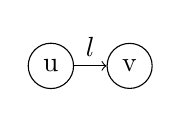
\begin{tikzpicture}
        \node[draw, circle] (x) at (0,0) {$\mathrm{u}$};
        \node[draw, circle] (y) at (1,0) {$\mathrm{v}$};
        \draw[->]  (x) -- (y) node [midway,above] {$l$};
    \end{tikzpicture} in the graph $T$,
    and $w(e) = 1.0$ for all $e \in \mathbb{E}$, can be visualized as follows:
    \begin{center}
        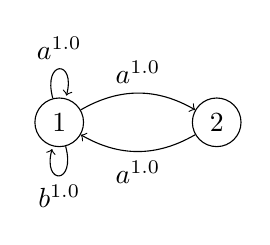
\begin{tikzpicture}
            \graphbox{}{0mm}{0mm}{32mm}{28mm}{-10mm}{-14mm}{
                \node[draw,circle] (1) at (0,0) {1};
                \node[draw,circle] (2) at (2,0) {2};
                \draw[->] (1) edge[loop above] node[midway, above] {$a^{1.0}$} (1) ;
                \draw[->] (1) edge[loop below] node[midway, below] {$b^{1.0}$} (1) ;
                \draw[->] (1) edge[bend left] node[midway, above] {$a^{1.0}$}  (2)  ;
                \draw[->] (2) edge[bend left] node[midway, below] {$a^{1.0}$} (1)   ;
            }
        \end{tikzpicture}
    \end{center}
\end{example}

\begin{example}
    Consider the following morphisms and the weighted type graph $\mathcal{T}$ from \autoref{example:weighted_type_graph}:
    \begin{center}
        \resizebox{0.49\textwidth}{!}{
        \begin{tikzpicture}
          \graphbox{\( L \)}{-50mm}{0mm}{40mm}{39mm}{2mm}{-6mm}{
            \coordinate (o) at (0mm,-10mm); 
            \node[draw,circle] (l1) at ($(o)+(-10mm,0mm)$) {1};
            \node[draw,circle] (l2) at ($(l1)+(2,0)$) {2};
            \node[draw,circle] (l3) at ($(l1) + (1,0)$) {3};
            \draw[] (l1) -- (l3) node[midway,above] {a};
            \draw[] (l3) -- (l2) node[midway,above] {a};
        } 
            \graphbox{$T$}{0mm}{0mm}{40mm}{39mm}{-10mm}{-17mm}{
                \node[draw,circle] (1) at (0,0) {$1\ 2$};
                \node[draw,circle] (2) at (2,0) {3};
                \draw[->] (1) edge[loop above] node[midway, above] {$a^{1.0}$} (1) ;
                \draw[->] (1) edge[loop below] node[midway, below] {$b^{1.0}$} (1) ;
                \draw[->] (1) edge[bend left] node[midway, above] {$a^{1.0}$}  (2)  ;
                \draw[->] (2) edge[bend left] node[midway, below] {$a^{1.0}$} (1)   ;
            }
            \node () at (-5mm,-15mm) {$\overset{h_{11}^1}{\to}$};
        \end{tikzpicture}
        }
        \resizebox{0.49\textwidth}{!}{
            \begin{tikzpicture}
              \graphbox{\(L\)}{-50mm}{0mm}{40mm}{39mm}{2mm}{-6mm}{
                \coordinate (o) at (0mm,-10mm); 
                \node[draw,circle] (l1) at ($(o)+(-10mm,0mm)$) {1};
                \node[draw,circle] (l2) at ($(l1)+(2,0)$) {2};
                \node[draw,circle] (l3) at ($(l1) + (1,0)$) {3};
                \draw[] (l1) -- (l3) node[midway,above] {a};
                \draw[] (l3) -- (l2) node[midway,above] {a};
            } 
                \graphbox{$T$}{0mm}{0mm}{40mm}{39mm}{-10mm}{-19mm}{
                    \node[draw,circle] (1) at (0,0) {$1\ 2\ 3$};
                    \node[draw,circle] (2) at (2,0) {};
                    \draw[->] (1) edge[loop above] node[midway, above] {$a^{1.0}$} (1) ;
                    \draw[->] (1) edge[loop below] node[midway, below] {$b^{1.0}$} (1) ;
                    \draw[->] (1) edge[bend left] node[midway, above] {$a^{1.0}$}  (2)  ;
                    \draw[->] (2) edge[bend left] node[midway, below] {$a^{1.0}$} (1)   ;(1)   ;
                }
                \node () at (-5mm,-15mm) {$\overset{h_{11}^2}{\to}$};
            \end{tikzpicture}
            }
      \end{center}
    We have $ w_\mathcal{T}(h_{11}^1) = w(e_{13a})^{m_{e_{13a}}(h_{11}^1)} \odot w(e_{31a})^{m_{e_{31a}}(h_{11}^1)} =
     1.0^1 * 1.0^1 = 1.0$ and $
        w_\mathcal{T}(h_{11}^2) 
        % = 1.0^1 * 1.0^1 
        = 1.0$
\end{example}

\subsection{Estimating weights of pushout objects}
Let \( \mathcal{R} = \mathcal{A} \cup \mathcal{B} \) be a set of DPO rewriting rules and let \(\mathcal{T} = (T, \mathbb{E}, \mathcal{S}, w)\) be a weighted type graph over the strongly monotonic measurable semiring $\mathcal{S}$. A proof of the following proposition can be found in \cite[Proposition 36]{qiu2025termination_nwf_v2_acceptedgcm}.

\begin{proposition}  
    % Let $\mathcal{S} = (S, \oplus, \odot, 0_\mathcal{S}, 1_\mathcal{S}, \prec, \mu)$ be a strongly monotonic measurable semiring. We have 
    For all $x,y$ in $\mathcal{S}$:
    \begin{align*}
        0_\mathcal{S} \neq x \land 0_\mathcal{S} \neq y 
        &\Rightarrow 0_\mathcal{S} \neq x \odot y 
        \\
        1_\mathcal{S} \preceq x \land 1_\mathcal{S} \preceq y \land 0_\mathcal{S} \neq x \land 0_\mathcal{S} \neq y  
        &\Rightarrow
         1_\mathcal{S} \preceq x \odot y 
         \\
         0_\mathcal{S} \neq x \land 0_\mathcal{S} \neq y   
         &\Rightarrow 0_\mathcal{S} \neq x \oplus y
    \end{align*}
\end{proposition}

    Suppose that (1) $w(e) \succeq 1_\mathcal{S}$ for all $e \in \mathbb{E}$, and (2) for all $x \in \mathcal{S}$, if $ 1_\mathcal{S} \preceq x \neq 0_\mathcal{S}$ then $\mu(x) \geq \mu(1_\mathcal{S})$ and $\mu(x) \in \mathbb{R}$. 
    By definition of a weighted type graph, $w(e)\neq 0_\mathcal{S}$ for all $e\in\mathbb{E}$.
    Therefore, by the proposition above, Hypothesis (1) and the definition of the weight of a morphism (\autoref{def:weight_of_a_morphism_relative_to_a_type_graph}), for all morphisms \( h \) from a finite graph $G$ to $\mathcal{T}$, we have \( 0_\mathcal{S} \neq w_\mathcal{T}(h) \succeq 1_\mathcal{S} \). 
    By the above proposition, Axiom \eqref{ax:s0} and the definition of the weight of an object (\autoref{def:weight_of_an_object_relative_to_a_type_graph}), we conclude that for all objects \( G \) with $\operatorname{Hom}(G,T)\neq \emptyset$, \( 0_\mathcal{S} \neq w_\mathcal{T}(G) \succeq 1_\mathcal{S} \). By Hypothesis (2), we have that for all objects \( G \) with $\operatorname{Hom}(G,T)\neq \emptyset$, \( \mu(w_\mathcal{T}(G)) \geq \mu(1_\mathcal{S}) = 0 \) if $\mathcal{S}$ is the real tropical or arctic semiring, and \( \mu(w_\mathcal{T}(G)) \geq 1 \) if $\mathcal{S}$ is the arithmetic semiring.

Suppose additionally that for every graph $G$ subject to rewriting, we have $\operatorname{Hom}(G,T)\neq \emptyset$. The rewriting relation \( \Rightarrow_{\mathcal{A},\mathfrak{F}} \) is terminating relative to $\Rightarrow_{\mathcal{B},\mathfrak{F}}$ if there exists a constant $\delta > 0$ such that: (i) for all \(G \Rightarrow_{\mathcal{A},\mathfrak{F}} H\), \( \mu(w_\mathcal{T}(G)) > \mu(w_\mathcal{T}(H)) + \delta \), and (ii) for all \(G \Rightarrow_{\mathcal{B},\mathfrak{F}} H\), \( \mu(w_\mathcal{T}(G)) \geq \mu(w_\mathcal{T}(H)) \). However, directly verifying all rewriting steps is infeasible due to the potentially infinite number of rewriting steps.
 
In this section, we recall the concepts of traceability of objects (Definition \ref{def:traceability}) and relative monicity of morphisms (\autoref{def:relative_monicity}), which are used to define the notion of weighable pushout squares (\autoref{def:weighable}). Using the notion of a weighable pushout square, we can bound the weight of the pushout object as explained below.  

\noindent
\begin{minipage}{0.7\textwidth}\setlength{\parindent}{1em}
    Consider a DPO diagram (illustrated on the right) that defines a rewriting step \( G \Rightarrow_{\rho,\mathfrak{F}} H \). 
    If the left pushout square is weighable with $\mathcal{T}$ and the right pushout square is bounded above by $\mathcal{T}$ (concepts defined in \autoref{def:weighable}), then, by \cite[Lemma 4.13]{endrullis2024generalized_arxiv_v2}, we obtain:
\end{minipage}%
\hfill
\begin{minipage}{0.29\textwidth}
    \hfill
    \resizebox{0.85\textwidth}{!}{
    \begin{tikzpicture}
        % [node distance=11mm]
        \node (I) at (0,0) {$K$};
        \node (L) at (-2,0) {$L$};
        \node (R) at (2,0) {$R$};
        \node (G) at (-2,-2) {$G$};
        \node (C) at (0,-2) {$C$};
        \node (H) at (2,-2) {$H$};
        \draw [->] (I) to  node [midway,below] {$l$} (L);
        \draw [->] (I) to  node [midway,below] {$r$} (R);
        \draw [->] (L) to node [midway,right] {$m$} (G);
        \draw [->] (I) to node [midway,right] {$u$} (C);
        \draw [->] (R) to node [midway,left] {$m'$} (H);
        \draw [->] (C) to node [midway,above] {$l'$} (G);
        \draw [->] (C) to node [midway,above] {$r'$} (H);
        \node [at=($(I)!.5!(G)$)] {\normalfont PO};
        \node [at=($(I)!.5!(H)$)] {\normalfont PO};
      \end{tikzpicture}
    }
\end{minipage}

% \begin{flalign*}
%     w_\mathcal{T}(G) 
%         & \overset{def}{=} \bigoplus_{t_G: G \rightarrow T} w_\mathcal{T}(t_G) 
%         \overset{def}{=} \bigoplus_{t_K: K \rightarrow T} \bigoplus_{\substack{t_G: G \rightarrow T\\ t_K = l \star m \star t_G}} w_\mathcal{T}(t_G) \\
%     w_\mathcal{T}(H) 
%         &\overset{def}{=} \bigoplus_{t_H: H \rightarrow T} w_\mathcal{T}(t_H) 
%          \overset{def}{=} \bigoplus_{t_K: K \rightarrow T} \bigoplus_{\substack{t_H: H \rightarrow T\\ t_K = r \star m' \star t_H}} w_\mathcal{T}(t_H)
% \end{flalign*}

% If the left pushout square is weighable with $\mathcal{T}$ and the right pushout square is bounded above by $\mathcal{T}$ (concepts defined in \autoref{def:weighable}), then, by \cite[Lemma 5.10]{endrullis2024generalized_lmcs}, we derive the following assertions:
% \begin{flalign*}
%     w_\mathcal{T}(G) 
%         & = \bigoplus_{t_K: K \rightarrow T} \bigoplus_{\substack{t_G: G \rightarrow T\\ t_K = l \star m \star t_G}} w_\mathcal{T}(m \star t_G) \odot (l' \star t_G - u) \\
%     w_\mathcal{T}(H) 
%         &  \preceq \bigoplus_{t_K: K \rightarrow T} \bigoplus_{\substack{t_H: H \rightarrow T\\ t_K = r \star m' \star t_H}} w_\mathcal{T}(m' \star t_H) \odot (r' \star t_H - u)
% \end{flalign*}
% By \cite[Theorem 5.12]{endrullis2024generalized_lmcs}, it follows:
% \begin{flalign*}
%     w_\mathcal{T}(G) 
%         & = \bigoplus_{t_K: K \rightarrow T} 
%         \bigoplus_{\substack{t_C: C \rightarrow T\\ t_K = u \star t_C}}
%         \bigoplus_{\substack{t_L: L \rightarrow T\\ t_K = l \star t_L}}
%             w_\mathcal{T}(t_L) \odot w_\mathcal{T}(t_C - u) \\
%     w_\mathcal{T}(H) 
%         &  \preceq \bigoplus_{t_K: K \rightarrow T} 
%         \bigoplus_{\substack{t_C: C \rightarrow T\\ t_K = u \star t_C}}
%         \bigoplus_{\substack{t_R: R \rightarrow T\\ t_K = r \star t_R}}
%             w_\mathcal{T}(t_R) \odot w_\mathcal{T}(t_C - u) \\
% \end{flalign*}
% By \cite[Theorem 5.13]{endrullis2024generalized_lmcs}, we have the following assertions: 
\begin{flalign*}
    w_\mathcal{T}(G) 
        & = \bigoplus_{t_K: K \rightarrow T} 
        \left ( \bigoplus_{\substack{t_C: C \rightarrow T\\ t_K = u \star t_C}}
          w_\mathcal{T}(t_C - u) \right ) 
          \odot
        \left (\bigoplus_{\substack{t_L: L \rightarrow T\\ t_K = l \star t_L}}
        w_\mathcal{T}(t_L) \right )
         \\
    w_\mathcal{T}(H) 
        &  \preceq \bigoplus_{t_K: K \rightarrow T} 
        \left ( \bigoplus_{\substack{t_C: C \rightarrow T\\ t_K = u \star t_C}}
         w_\mathcal{T}(t_C - u) \right ) 
         \odot 
         \left ( \bigoplus_{\substack{t_R: R \rightarrow T\\ t_K = r \star t_R}}
            w_\mathcal{T}(t_R) \right ) \\
\end{flalign*}
According to these results, a termination criterion will be established in \autoref{sec:nwf:termination} by comparing the weights 
$\bigoplus_{\substack{t_L: L \rightarrow T\\ t_K = l \star t_L}}
        w_\mathcal{T}(t_L)$ and 
$\bigoplus_{\substack{t_R: R \rightarrow T\\ t_K = r \star t_R}} 
        w_\mathcal{T}(t_R)$ for every $t_K: K \rightarrow T$.

\subsection{Decreasing rules}
\label{sec:nwf:decreasing_rules}
The definition below adapts the concept of decreasing rules from~\cite{endrullis2024generalized_arxiv_v2}. The difference lies in the treatment of weight comparisons for uniformly decreasing and closure decreasing rules: instead of directly comparing weights, we evaluate the difference between weights relative to the homomorphism $\mu$ of the strongly monotonic measurable semirings.
%  This difference must exceed a fixed positive constant $\delta \in \mathbb{R}_{>0}$.

\begin{definition}[Decreasing Rules]
    \label{def:nwf:decreasing_rule}
    Let $\mathcal{T} = (T,\mathbb{E}, (S, \oplus, \odot, 0_S, 1_S, \prec, \mu), w)$ be a finitary weighted type graph, \(\mathfrak{F}\) a DPO rewriting framework, $\rho = (L \overset{l}{\leftarrow} K \overset{r}{\rightarrow} R)$ a DPO rewriting rule, and $\delta \in \mathbb{R}_{>0}$. 

    \noindent
    The rule $\rho$ is \textbf{weakly decreasing} w.r.t. $\mathcal{T}$ in $\mathfrak{F}$ if 
            for every $t_K : K \to T$,
                $$ 
                  w_\mathcal{T}(\{l \star - = t_K\}) \succeq w_\mathcal{T}(\{r\star - = t_K\})$$
           
    \noindent
    The rule $\rho$ is \textbf{$\delta$-uniformly decreasing} w.r.t. $\mathcal{T}$ in $\mathfrak{F}$ if the following hold:
        \begin{itemize}
            \item[]- there exists a context closure $c_\rho$ for $\rho$ and $\mathcal{T}$ in $\mathfrak{F}$, 
            \item[]- for every $t_K : K \to T$,
            \begin{itemize}
                \item[] $\bullet$ $\{l \star - = t_K\} = \emptyset = \{r \star - = t_K\}$, or
                \item[] $\bullet$ $\mu(w_\mathcal{T}(\{l \star - = t_K\}))  >   \mu(w_\mathcal{T}(\{r \star - = t_K\})) + \delta$.
            \end{itemize}
        \end{itemize}  
         
    \noindent
    The rule $\rho$ is
            \textbf{$\delta$-closure decreasing} w.r.t. $\mathcal{T}$ in $\mathfrak{F}$ if the following hold:
            \begin{itemize}
                \item[]- $S$ is strictly monotonic measurable semiring,
                \item[]- $\rho$ is weakly decreasing,
                \item[]- there exists a context closure $c_\rho$ for $\rho$ and $\mathcal{T}$ in $\mathfrak{F}$,
                \item[]- $ \mu(w_\mathcal{T}(\{l \star - = t_K\}))  >  \mu(w_\mathcal{T}(\{r \star - = t_K\}))  + \delta$ for $t_K = l \star c_\rho$.
            \end{itemize}
\end{definition}

\begin{example}
    \label{example:nwf:decreasing_rule}
    Consider the DPO rule in \autoref{ex:grsaa} and the weighted type graph in \autoref{example:weighted_type_graph} over the real arithmetic semiring $\mathfrak{N}' = (\mathbb{R}^+,+,*,0_\mathbb{R},1_\mathbb{R},<,\operatorname{id}_{\mathbb{R}^+})$. There are $t_K^{11}, t_K^{12}, t_K^{21}, t_K^{22}:K \rightarrow T$ as depicted below:

    \begin{center}
        \resizebox{0.49\textwidth}{!}{
            \begin{tikzpicture}
            \graphbox{\( K \)}{-50mm}{0mm}{40mm}{30mm}{2mm}{-6mm}{
                \coordinate (o) at (0mm,-10mm); 
                \node[draw,circle] (l1) at ($(o)+(-10mm,0mm)$) {1};
                \node[draw,circle] (l2) at ($(l1)+(2,0)$) {2};
                % \node[draw,circle] (l3) at ($(l1) + (1,0)$) {3};
                % \draw[] (l1) -- (l3) node[midway,above] {a};
                % \draw[] (l3) -- (l2) node[midway,above] {a};
            } 
                \graphbox{$T$}{0mm}{0mm}{40mm}{30mm}{-10mm}{-15mm}{
                    \node[draw,circle] (1) at (0,0) {$1\ 2$};
                    \node[draw,circle] (2) at (2,0) {};
                    \draw[->] (1) edge[loop above] node[midway, above] {$a$} (1) ;
                    \draw[->] (1) edge[loop below] node[midway, below] {$b$} (1) ;
                    \draw[->] (1) edge[bend left] node[midway, above] {$a$}  (2)  ;
                    \draw[->] (2) edge[bend left] node[midway, below] {$a$} (1)   ;
                }
                \node () at (-5mm,-15mm) {$\overset{t_K^{11}}{\to}$};
            \end{tikzpicture}
            } 
            \resizebox{0.49\textwidth}{!}{
            \begin{tikzpicture}
                \graphbox{\( K \)}{-50mm}{0mm}{40mm}{30mm}{2mm}{-6mm}{
                \coordinate (o) at (0mm,-10mm); 
                \node[draw,circle] (l1) at ($(o)+(-10mm,0mm)$) {1};
                \node[draw,circle] (l2) at ($(l1)+(2,0)$) {2};
                % \node[draw,circle] (l3) at ($(l1) + (1,0)$) {3};
                % \draw[] (l1) -- (l3) node[midway,above] {a};
                % \draw[] (l3) -- (l2) node[midway,above] {a};
            } 
                \graphbox{$T$}{0mm}{0mm}{40mm}{30mm}{-10mm}{-15mm}{
                    \node[draw,circle] (1) at (0,0) {$1$};
                    \node[draw,circle] (2) at (2,0) {2};
                    \draw[->] (1) edge[loop above] node[midway, above] {$a$} (1) ;
                    \draw[->] (1) edge[loop below] node[midway, below] {$b$} (1) ;
                    \draw[->] (1) edge[bend left] node[midway, above] {$a$}  (2)  ;
                    \draw[->] (2) edge[bend left] node[midway, below] {$a$} (1)   ;
                }
                \node () at (-5mm,-15mm) {$\overset{t_K^{12}}{\to}$};
            \end{tikzpicture}
            }
            \hspace{5mm}
            
            \resizebox{0.49\textwidth}{!}{
            \begin{tikzpicture}
                \graphbox{\( K \)}{-50mm}{0mm}{40mm}{30mm}{2mm}{-6mm}{
                \coordinate (o) at (0mm,-10mm); 
                \node[draw,circle] (l1) at ($(o)+(-10mm,0mm)$) {1};
                \node[draw,circle] (l2) at ($(l1)+(2,0)$) {2};
                % \node[draw,circle] (l3) at ($(l1) + (1,0)$) {3};
                % \draw[] (l1) -- (l3) node[midway,above] {a};
                % \draw[] (l3) -- (l2) node[midway,above] {a};
            } 
                \graphbox{$T$}{0mm}{0mm}{40mm}{30mm}{-10mm}{-15mm}{
                    \node[draw,circle] (1) at (0,0) {2};
                    \node[draw,circle] (2) at (2,0) {1};
                    \draw[->] (1) edge[loop above] node[midway, above] {$a$} (1) ;
                    \draw[->] (1) edge[loop below] node[midway, below] {$b$} (1) ;
                    \draw[->] (1) edge[bend left] node[midway, above] {$a$}  (2)  ;
                    \draw[->] (2) edge[bend left] node[midway, below] {$a$} (1)   ;
                }
                \node () at (-5mm,-15mm) {$\overset{t_K^{21}}{\to}$};
            \end{tikzpicture}
            }
            \resizebox{0.49\textwidth}{!}{
            \begin{tikzpicture}
                \graphbox{\( K \)}{-50mm}{0mm}{40mm}{30mm}{2mm}{-6mm}{
                \coordinate (o) at (0mm,-10mm); 
                \node[draw,circle] (l1) at ($(o)+(-10mm,0mm)$) {1};
                \node[draw,circle] (l2) at ($(l1)+(2,0)$) {2};
                % \node[draw,circle] (l3) at ($(l1) + (1,0)$) {3};
                % \draw[] (l1) -- (l3) node[midway,above] {a};
                % \draw[] (l3) -- (l2) node[midway,above] {a};
            } 
                \graphbox{$T$}{0mm}{0mm}{40mm}{30mm}{-10mm}{-15mm}{
                    \node[draw,circle] (1) at (0,0) {};
                    \node[draw,circle] (2) at (2,0) {$1\ 2$};
                    \draw[->] (1) edge[loop above] node[midway, above] {$a$} (1) ;
                    \draw[->] (1) edge[loop below] node[midway, below] {$b$} (1) ;
                    \draw[->] (1) edge[bend left] node[midway, above] {$a$}  (2)  ;
                    \draw[->] (2) edge[bend left] node[midway, below] {$a$} (1)   ;
                }
                \node () at (-5mm,-15mm) {$\overset{t_K^{22}}{\to}$};
            \end{tikzpicture}
            }
      \end{center}
    The set $\{l \star - = t_K^{11}\}$ has two morphisms $h_{11}^1$ and $h_{11}^2$ as illustrated below:
    \begin{center}
        \resizebox{0.49\textwidth}{!}{
        \begin{tikzpicture}
          \graphbox{\( L \)}{-50mm}{0mm}{40mm}{40mm}{2mm}{-6mm}{
            \coordinate (o) at (0mm,-10mm); 
            \node[draw,circle] (l1) at ($(o)+(-10mm,0mm)$) {1};
            \node[draw,circle] (l2) at ($(l1)+(2,0)$) {2};
            \node[draw,circle] (l3) at ($(l1) + (1,0)$) {3};
            \draw[] (l1) -- (l3) node[midway,above] {a};
            \draw[] (l3) -- (l2) node[midway,above] {a};
        } 
            \graphbox{$T$}{0mm}{0mm}{40mm}{40mm}{-10mm}{-17mm}{
                \node[draw,circle] (1) at (0,0) {$1\ 2$};
                \node[draw,circle] (2) at (2,0) {3};
                \draw[->] (1) edge[loop above] node[midway, above] {$a^{1.0}$} (1) ;
                \draw[->] (1) edge[loop below] node[midway, below] {$b^{1.0}$} (1) ;
                \draw[->] (1) edge[bend left] node[midway, above] {$a^{1.0}$}  (2)  ;
                \draw[->] (2) edge[bend left] node[midway, below] {$a^{1.0}$} (1)   ;
            }
            \node () at (-5mm,-15mm) {$\overset{h_{11}^1}{\to}$};
        \end{tikzpicture}
        }
        \resizebox{0.49\textwidth}{!}{
            \begin{tikzpicture}
              \graphbox{\(L\)}{-50mm}{0mm}{40mm}{40mm}{2mm}{-10mm}{
                \coordinate (o) at (0mm,-10mm); 
                \node[draw,circle] (l1) at ($(o)+(-10mm,0mm)$) {1};
                \node[draw,circle] (l2) at ($(l1)+(2,0)$) {2};
                \node[draw,circle] (l3) at ($(l1) + (1,0)$) {3};
                \draw[] (l1) -- (l3) node[midway,above] {a};
                \draw[] (l3) -- (l2) node[midway,above] {a};
            } 
                \graphbox{$T$}{0mm}{0mm}{40mm}{40mm}{-10mm}{-20mm}{
                    \node[draw,circle] (1) at (0,0) {$1\ 2\ 3$};
                    \node[draw,circle] (2) at (2,0) {};
                    \draw[->] (1) edge[loop above] node[midway, above] {$a^{1.0}$} (1) ;
                    \draw[->] (1) edge[loop below] node[midway, below] {$b^{1.0}$} (1) ;
                    \draw[->] (1) edge[bend left] node[midway, above] {$a^{1.0}$}  (2)  ;
                    \draw[->] (2) edge[bend left] node[midway, below] {$a^{1.0}$} (1)   ;(1)   ;
                }
                \node () at (-5mm,-15mm) {$\overset{h_{11}^2}{\to}$};
            \end{tikzpicture}
            }
      \end{center}
    Therefore, we have \begin{flalign*}
        w_\mathcal{T}(\{l \star - = t_K^{11}\})
        =&w_\mathcal{T}(\{h_{11}^1, h_{11}^2\})\\
        \overset{\mathrm{def}}{=}&w_\mathcal{T}(h_{11}^1) + w_\mathcal{T}(h_{11}^2) \\
        =&(1.0^1 * 1.0^1) + (1.0^1 * 1.0^1)\\
        =&2.0
    \end{flalign*}
    The set $\{r \star - = t_K^{11}\}$ has one morphism $h_{11}^3$ as illustrated below:
    \begin{center}
        \resizebox{0.49\textwidth}{!}{
        \begin{tikzpicture}
          \graphbox{\( R \)}{-55mm}{0mm}{45mm}{44mm}{1mm}{-22mm}{
            \coordinate (o) at (-5mm,-3mm); 
            \node[draw,circle] (l1) at ($(o)+(-10mm,0mm)$) {1};
            \node[draw,circle] (l2) at ($(l1)+(3,0)$) {2};
            \node[draw,circle] (l3) at ($(l1) + (1,0)$) {4};
            \node[draw,circle] (l4) at ($(l1) + (2,0)$) {5};
            \draw[->] (l1) -- (l3) node[midway,above] {a};
            \draw[->] (l3) -- (l4) node[midway,above] {b};
            \draw[->] (l4) -- (l2) node[midway,above] {a};
        } 
            \graphbox{$T$}{0mm}{0mm}{40mm}{44mm}{-10mm}{-22mm}{
                \node[draw,circle] (1) at (0,0) {$1\ 2\ 4\ 5$};
                \node[draw,circle] (2) at (2,0) {};
                \draw[->] (1) edge[loop above] node[midway, above] {$a^{1.0}$} (1) ;
                \draw[->] (1) edge[loop below] node[midway, below] {$b^{1.0}$} (1) ;
                \draw[->] (1) edge[bend left] node[midway, above] {$a^{1.0}$}  (2)  ;
                \draw[->] (2) edge[bend left] node[midway, below] {$a^{1.0}$} (1)   ;
            }
            \node () at (-5mm,-19mm) {$\overset{h_{11}^3}{\to}$};
        \end{tikzpicture}
        }
      \end{center}
    Therefore, we have: $w_\mathcal{T}(\{r \star - = t_K^{11}\}) = w_\mathcal{T}(h_{11}^3) = 1.0^1 * 1.0^1 * 1.0 ^ 1 = 1.0$. Thus, we have $w_\mathcal{T}(\{l \star - = t_K^{11}\}) = 2.0 \geq 1.0 = w_\mathcal{T}(\{r \star - = t_K^{11}\})$.

    Similarly, we can check that $w_\mathcal{T}(\{l \star - = t_K^{12}\}) = 1.0 \geq 1.0 = w_\mathcal{T}(\{r \star - = t_K^{12}\})$,  $w_\mathcal{T}(\{l \star - = t_K^{21}\}) = 1.0 \geq 1.0 = w_\mathcal{T}(\{r \star - = t_K^{21}\})$, and $w_\mathcal{T}(\{l \star - = t_K^{22}\}) = 1.0 \geq 1.0 = w_\mathcal{T}(\{r \star - = t_K^{22}\})$. The rule is therefore weakly decreasing.

    There exists a context closure $c$ for the DPO rule in the weighted type graph, as shown in \autoref{example:context_closure}.
    Since we have additionally $t_K^{11} = l \star c$ and $w_\mathcal{T}(\{l \star - = t_K^{11}\}) = 2.0 > 1.0 + \delta = w_\mathcal{T}(\{r \star - = t_K^{11}\}) + \delta$ for $0 < \delta < 1.0$, the rule is $\delta$-closure decreasing with $0 < \delta < 1.0$ since the semiring is strictly monotonic measurable.
\end{example} 

Adapted from \cite[Theorem C.3]{endrullis2024generalized_arxiv_v2}, the lemma below relates decreasing rules to weight reduction under specific constraints. 
For its proof, we refer to \cite[Theorem 36]{qiu2025termination_nwf_v2_acceptedgcm}.
\begin{lemma}[Decreasing steps]
    \label{lem:decreasing_step}
\ \newline
\begin{minipage}{0.7\textwidth}
    Let $\mathcal{T} = (T,\mathbb{E}, (S, \oplus, \odot, 0_S, 1_S, \prec, \mu), w)$ be a finitary weighted type graph, $\rho$ a rewriting rule and $\Delta \in \mathfrak{F}(\rho)$ a DPO diagram
    (shown on the right)   such that the following conditions hold:
\end{minipage}  
\begin{minipage}{0.3\textwidth}
    \begin{center}
        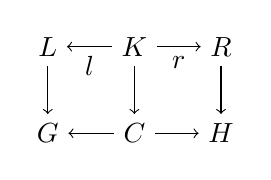
\begin{tikzpicture}[node distance=11mm]
          \node (I) {$K$};
          \node (L) [left of= I] {$L$};
          \node (R) [right of=I] {$R$}; 
          \node (G) [below of=L] {$G$};
          \node (C) [below of=I] {$C$};
          \node (H) [below of=R] {$H$};
        %   \node (T) [left=of $(L)!0.5!(G)$] {$T$};
        %   \draw [->] (L) to  node [label, above] {$c$}  (T);
        %   \draw [->] (G) to  node [label, below] {$\alpha$} (T);
          \draw [->] (I) to node [label, below] {$l$} (L);
          \draw [->] (I) to node [label, below] {$r$} (R);
          \draw [->] (L) to  (G);
          \draw [->] (I) to (C);
          \draw [->] (R) to (H);
          \draw [->] (C) to (G);
          \draw [->] (C) to (H);
        \end{tikzpicture}
      \end{center}
\end{minipage}
   \begin{itemize}
       \item $\operatorname{left}(\Delta)$ is weighable with \(\mathcal{T}\), and
       \item $\operatorname{right}(\Delta)$ is bounded above by \(\mathcal{T}\), and
       \item $w(e) \succeq 1_S$ for all $e \in \mathbb{E}$.
   \end{itemize}

   \noindent
  We have:
   \begin{itemize}
       \item $\mu(w_\mathcal{T}(G)) \succeq \mu(w_\mathcal{T}(H))$ if $\rho$ is weakly decreasing,
       \item $\mu(w_\mathcal{T}(G)) > \mu(w_\mathcal{T}(H)) + \delta$ if $\rho$ is $\delta$-uniformly or $\delta$-closure decreasing for some $\delta >0$ and $w(e) \succeq 1_S$ for all $e \in \mathbb{E}$.
   \end{itemize}
\end{lemma} 
% \begin{proof}
%    See the \hyperref[proof:decreasing_step]{Appendix}.
% \end{proof}

\subsection{Termination Criterion}
\label{sec:nwf:proving_termination}
Finally, we formulate a termination criterion leveraging type graphs weighted over non-well-founded semirings. For its proof, we refer to \cite[Theorem 37]{qiu2025termination_nwf_v2_acceptedgcm}.
\begin{theorem}[Termination of DPO rewriting system] 
    \label{thm:termination_grs}
    Let $\mathcal{A}$ and $\mathcal{B}$ be sets of DPO rewriting rules, $\mathcal{T} = (T,\mathbb{E}, (S, \oplus, \odot, 0_S, 1_S, \prec, \mu), w)$ a finitary weighted type graph and $\mathfrak{F}$ a DPO rewriting framework such that

     \begin{enumerate}[label=\roman*)]
        \item\label{thm1:hyp3} $w(e) \succeq 1_S$ for all $e \in \mathbb{E}$, and
        % \item\label{thm1:hyp4} $\{s \in S\mid 1_S \leq s \neq 0_S\} \subseteq \mathbb{R}_{>0}$ 
        % \item\label{thm1:hyp4} for all $x \in S$, if $ 1_S \preceq x \neq 0_S$ then $\mu(x) \geq \mu(1_S)$ and $\mu(x) \in \mathbb{R}$,
        \item\label{thm1:hyp4} for all $x \in S$, if $ 1_S \preceq x \neq 0_S$ then $\mu(x) \geq \mu(1_S)$ and $\mu(x) \in \mathbb{R}$, and
        \item for every rule $\rho \in (\mathcal{A }\cup \mathcal{B })$ and every double pushout diagram  
        $\Delta \in \mathfrak{F}(\rho)$ 
        \begin{itemize}
            \item \(\operatorname{left}(\Delta)\) is weighable with \(\mathcal{T}\),
            \item \(\operatorname{right}(\Delta)\) is bounded above by \(\mathcal{T}\). 
        \end{itemize}
    \end{enumerate}       

    \noindent If the following conditions hold:
    \begin{enumerate}
        \item there exists $\delta >0$ such that either every $\rho \in \mathcal{A}$ is $\delta$-uniformly decreasing, or every $\rho \in \mathcal{A}$ is $\delta$-closure decreasing, and
        \item every rule $\rho \in \mathcal{B}$ is weakly decreasing,
    \end{enumerate}
    then $\Rightarrow_{\mathcal{A},\mathfrak{F}}$ is \textbf{terminating} relative to $\Rightarrow_{\mathcal{B},\mathfrak{F}}$.
\end{theorem} 
% \begin{proof}
%     See the \hyperref[proof_termination_grs]{Appendix}.
% \end{proof}
\begin{example}
    \label{example:termination}
    Termination of the DPO rule in \autoref{ex:grsaa} can be established using \autoref{thm:termination_grs} together with the weighted type graph in \autoref{example:weighted_type_graph} over the real arithmetic semiring $\mathfrak{N}' = (\mathbb{R}^+,+,*,0_\mathbb{R},1_\mathbb{R},<,\operatorname{id}_{\mathbb{R}^+})$. It is $\delta$-closure decreasing with $\delta = 0.5$ by \autoref{example:decreasing_rule}.
\end{example}

